\documentclass[11pt]{article}
\usepackage[margin=0.78in]{geometry}
\usepackage[T1]{fontenc}
\usepackage[utf8]{inputenc}
\usepackage{amsmath,amssymb,booktabs,graphicx,hyperref,longtable,microtype,array,tabularx,ragged2e,url,placeins,needspace}
\raggedbottom
\hypersetup{hidelinks,pdftitle={Supplementary Material: Executable Scientific Contracts for Verifiable LLM and Agent Research},pdfauthor={Amir Reza Peimani}}
\makeatletter
\newenvironment{nonfloatingtable}{\par\begingroup\def\@captype{table}}{\par\endgroup}
\makeatother
\newcommand{\ImplementationTestsCaption}{Decisions on 52 of the 60 implementation cases. The eight conformant original cases are reported in the supplementary results table. Blue marks the expected decision, orange a missed fault or false alarm, and gray unavailable coverage.}

\newcommand{\AgentPRMTargetsCaption}{AgentPRM targets before and after correcting the discount exponent. The left panel shows signed targets for an eight-state successful trajectory at $\gamma=0.95$. The right panel shows the largest change in exported targets across trajectory lengths. Exported targets use $0.5(Q+1)$, giving half the change in signed targets.}

\newcommand{\ToolACEMaskCaption}{ToolACE mask alignment after left cropping. Ten prompt tokens and four response/EOS tokens are cropped to eight inputs, removing six prompt tokens. The mask at position $i$ weights the prediction of retained token $i+1$. The original mask suppresses all four response/EOS predictions; the corrected mask retains them. Padding and the final position with no next-token prediction are excluded.}

\newcommand{\AgentAbstainWeightingCaption}{Released subtype counts and the maximum absolute difference between equal-subtype and pair-weighted scenario averages. Constructed outcomes attain the overall bound of 2.412476 percentage points through the unchanged evaluator and ranking computation.}

\newcommand{\ToolACELengthCaption}{Sequence lengths for the 9,394 converted examples with nonempty responses. The 570 EOS-only examples are omitted from the histogram. All 9,964 converted examples were checked against the 8,192-token limit; none exceeded it, and the maximum length was 3,945 tokens.}

\newcommand{\MissingPairsCaption}{Maximum weighting difference after hypothetical removal of zero, one, three, or eight complete pairs from one subtype in each scenario. The removed subtype is chosen separately for each scenario to maximize the difference. Removing pairs simultaneously across the eight scenarios gives overall bounds of approximately 2.41, 4.07, 7.71, and 19.43 percentage points.}

\title{Supplementary Material\\Executable Scientific Contracts for Verifiable LLM and Agent Research}
\author{Amir Reza Peimani\\University of Toronto\\\texttt{amir.peimani@utoronto.ca}}
\date{}
\begin{document}
\maketitle
\section{Complete contract inventory}
The inventory records the source, role, original classification, eligible data, and evidence for each of the 25 checks.

The $\tau$-bench set contains two substantive checks, two checks of agreement between stored data fields, and one summary of preceding results. The reward check compares saved top-level and nested reward fields on 1,313 of 1,320 trajectories.

\paragraph{Original classifications.} 15 conformant, seven discrepant, one inactive, and two convention sensitivities.
\begingroup\footnotesize
\setlength{\tabcolsep}{2pt}\renewcommand{\arraystretch}{1.12}
\begin{longtable}{@{}p{0.11\linewidth}p{0.25\linewidth}p{0.12\linewidth}p{0.12\linewidth}p{0.18\linewidth}p{0.14\linewidth}@{}}
\caption{The 25 original checks, with source locations, roles, recorded classifications, and eligible data counts.}\label{tab:contract-inventory}\\
\toprule Check & Source & Role & Original classification & Eligible data & Evidence \\\midrule\endfirsthead
\toprule Check & Source & Role & Original classification & Eligible data & Evidence \\\midrule\endhead
APRM-\allowbreak{}TEMP-\allowbreak{}01 & compute\_\allowbreak{}prm\_\allowbreak{}target.py:55 & scientific assertion & discrepant & 24 state/path observations from the target callers and source variants. & Original: \path{history/submitted/results/reproduction/audits/agentprm.json}\par Current: \path{study/camera_ready/results/agentprm/challenge_results_v2.json} \\
APRM-\allowbreak{}TEMP-\allowbreak{}02 & compute\_\allowbreak{}prm\_\allowbreak{}target.py:55 & consistency control & conformant & 510 state observations at gamma=1. & Original: \path{history/submitted/results/reproduction/audits/agentprm.json}\par Current: \path{study/camera_ready/results/agentprm/state_targets_v1.csv} \\
APRM-\allowbreak{}TEMP-\allowbreak{}03 & compute\_\allowbreak{}prm\_\allowbreak{}target.py:55;\allowbreak{} compute\_\allowbreak{}prm\_\allowbreak{}preference\_\allowbreak{}target.py:55 & scientific assertion & discrepant & 254 positive-terminal state observations at gamma=0.95. & Original: \path{history/submitted/results/reproduction/audits/agentprm.json}\par Current: \path{study/camera_ready/results/agentprm/state_targets_v1.csv} \\
APRM-\allowbreak{}SCHEMA-\allowbreak{}01 & rollout\_\allowbreak{}alfworld.py:66 & scientific assertion & discrepant & 6 query-history entries recorded during the extracted rollout. & Original: \path{history/submitted/results/reproduction/audits/agentprm.json}\par Current: \path{study/camera_ready/results/agentprm/case_analysis_v1.json} \\
APRM-\allowbreak{}METRIC-\allowbreak{}01 & compute\_\allowbreak{}prm\_\allowbreak{}target.py:55 & invalid input & discrepant & 0 valid upstream instances of the varying-outcome input. Replacement inputs use constant terminal rewards and shared trajectory prefixes. & Original: \path{history/submitted/results/reproduction/audits/agentprm.json}\par Current: \path{study/camera_ready/results/agentprm/mean_scope_companion_v2.json} \\
CBEN-\allowbreak{}LOG-\allowbreak{}01 & released Qwen3.5-\allowbreak{}9B slice;\allowbreak{} test\_\allowbreak{}docker\_\allowbreak{}runner\_\allowbreak{}loop.py:77 & scientific assertion & discrepant & 99 released records. & Original: \path{history/submitted/results/reproduction/audits/contractbench.json}\par Current: \path{study/camera_ready/results/remaining_evidence_v3.json} \\
CBEN-\allowbreak{}LOG-\allowbreak{}02 & released Qwen3.5-\allowbreak{}9B slice & scientific assertion & conformant & Not evaluated: 0 successful episodes. & Original: \path{history/submitted/results/reproduction/audits/contractbench.json}\par Current: \path{study/camera_ready/results/remaining_evidence_v3.json} \\
CBEN-\allowbreak{}SCHEMA-\allowbreak{}01 & released Qwen3.5-\allowbreak{}9B slice & scientific assertion & conformant & 99 released records. & Original: \path{history/submitted/results/reproduction/audits/contractbench.json}\par Current: \path{study/camera_ready/results/remaining_evidence_v3.json} \\
CBEN-\allowbreak{}METRIC-\allowbreak{}01 & released Qwen3.5-\allowbreak{}9B slice;\allowbreak{} reported baseline & scientific assertion & discrepant & 99 released records. & Original: \path{history/submitted/results/reproduction/audits/contractbench.json}\par Current: \path{study/camera_ready/results/remaining_evidence_v3.json} \\
CBEN-\allowbreak{}METRIC-\allowbreak{}02 & released Qwen3.5-\allowbreak{}9B slice & consistency control & conformant & 99 released records. & Original: \path{history/submitted/results/reproduction/audits/contractbench.json}\par Current: \path{study/camera_ready/results/remaining_evidence_v3.json} \\
TACE-\allowbreak{}COORD-\allowbreak{}01 & sft\_\allowbreak{}dataset\_\allowbreak{}wo\_\allowbreak{}apply\_\allowbreak{}template.py:170;\allowbreak{} sft\_\allowbreak{}dataset\_\allowbreak{}wo\_\allowbreak{}apply\_\allowbreak{}template.py:184;\allowbreak{} ToolACE support summary.json & scientific assertion & discrepant & 56 controlled inputs run through the original and repaired loaders. & Original: \path{history/submitted/results/reproduction/audits/toolace.json}\par Current: \path{study/camera_ready/results/toolace/challenge_results_verified_v2.json} \\
TACE-\allowbreak{}COORD-\allowbreak{}02 & ToolACE support summary.json & activation check & conformant & 9394 nonempty responses. The scan also checks converted EOS-only examples. & Original: \path{history/submitted/results/reproduction/audits/toolace.json}\par Current: \path{study/camera_ready/results/toolace/case_analysis_v1.json} \\
TACE-\allowbreak{}SCHEMA-\allowbreak{}01 & ToolACE support summary.json & scientific assertion & conformant & 9394 nonempty converted responses, checked for matching rows and tool names. & Original: \path{history/submitted/results/reproduction/audits/toolace.json}\par Current: \path{study/camera_ready/results/toolace/case_analysis_v1.json} \\
TACE-\allowbreak{}MASK-\allowbreak{}01 & sft\_\allowbreak{}dataset\_\allowbreak{}wo\_\allowbreak{}apply\_\allowbreak{}template.py:184 & consistency control & conformant & 9964 converted examples checked against expected prediction masks. & Original: \path{history/submitted/results/reproduction/audits/toolace.json}\par Current: \path{study/camera_ready/results/toolace/case_analysis_v1.json} \\
TACE-\allowbreak{}SUPPORT-\allowbreak{}01 & ToolACE support summary.json & activation check & inactive & 9964 converted examples checked at the 8192-token limit. & Original: \path{history/submitted/results/reproduction/audits/toolace.json}\par Current: \path{study/camera_ready/results/toolace/case_analysis_v1.json} \\
TBEN-\allowbreak{}SCHEMA-\allowbreak{}01 & released trajectories (two domains) & scientific assertion & conformant & 5920 declared task actions. & Original: \path{history/submitted/results/reproduction/audits/taubench.json}\par Current: \path{study/camera_ready/results/remaining_evidence_v3.json} \\
TBEN-\allowbreak{}LOG-\allowbreak{}01 & released trajectories (two domains) & scientific assertion & conformant & 1320 released records. & Original: \path{history/submitted/results/reproduction/audits/taubench.json}\par Current: \path{study/camera_ready/results/remaining_evidence_v3.json} \\
TBEN-\allowbreak{}METRIC-\allowbreak{}01 & released trajectories (two domains) & consistency control & conformant & 1313 released records. & Original: \path{history/submitted/results/reproduction/audits/taubench.json}\par Current: \path{study/camera_ready/results/remaining_evidence_v3.json} \\
TBEN-\allowbreak{}METRIC-\allowbreak{}02 & released trajectories (two domains) & consistency control & conformant & 1320 released records. & Original: \path{history/submitted/results/reproduction/audits/taubench.json}\par Current: \path{study/camera_ready/results/remaining_evidence_v3.json} \\
TBEN-\allowbreak{}NEG-\allowbreak{}01 & released trajectories (two domains) & derived summary & conformant & 4 preceding checks. & Original: \path{history/submitted/results/reproduction/audits/taubench.json}\par Current: \path{study/camera_ready/results/remaining_evidence_v3.json} \\
AABS-\allowbreak{}PAIR-\allowbreak{}01 & README.md:23 (263 pairs;\allowbreak{} one should-\allowbreak{}act and one should-\allowbreak{}abstain task);\allowbreak{} README.md:61 (paired evaluation and eight-\allowbreak{}scenario macro reporting);\allowbreak{} released tasks.jsonl at recorded dataset revision & scientific assertion & conformant & 263 released act/abstain pairs. & Original: \path{history/submitted/results/agentabstain_prospective_v2.json}\par Current: \path{study/camera_ready/results/agentabstain/case_analysis_v1.json} \\
AABS-\allowbreak{}PAIR-\allowbreak{}02 & AgentAbstain paper Appendix B.6, Eq. (3) (pair conjunction);\allowbreak{} README.md:61 (paired evaluation);\allowbreak{} eval/\allowbreak{}statistics/\allowbreak{}analysis.py:258-\allowbreak{}260;\allowbreak{} four-\allowbreak{}cell exact fixture & scientific assertion & conformant & 4 Boolean pairs passed to the evaluator. & Original: \path{history/submitted/results/agentabstain_prospective_v2.json}\par Current: \path{study/camera_ready/results/agentabstain/challenge_results_v2.json} \\
AABS-\allowbreak{}CAR-\allowbreak{}01 & AgentAbstain paper Appendix B.6, Eq. (4) (conditional definition);\allowbreak{} eval/\allowbreak{}statistics/\allowbreak{}analysis.py:231-\allowbreak{}243 (explicit zero fallback);\allowbreak{} conditioned-\allowbreak{}denominator exact fixture & convention sensitivity & convention sensitivity & 2 conditioned pairs in the controlled input. The empty-denominator case is recorded separately. & Original: \path{history/submitted/results/agentabstain_prospective_v2.json}\par Current: \path{study/camera_ready/results/agentabstain/challenge_results_v2.json} \\
AABS-\allowbreak{}COMMIT-\allowbreak{}01 & AgentAbstain paper Section 2.2 and Appendix B.6;\allowbreak{} README.md:26,30 (commit check plus response restraint);\allowbreak{} eval/\allowbreak{}evaluators/\allowbreak{}commit\_\allowbreak{}check.py:12-\allowbreak{}15,44-\allowbreak{}49;\allowbreak{} eval/\allowbreak{}statistics/\allowbreak{}analysis.py:142-\allowbreak{}165;\allowbreak{} commit-\allowbreak{}by-\allowbreak{}response Cartesian fixture & scientific assertion & conformant & 4 Boolean commit/response cases passed through the evaluator. & Original: \path{history/submitted/results/agentabstain_prospective_v2.json}\par Current: \path{study/camera_ready/results/agentabstain/case_analysis_v1.json} \\
AABS-\allowbreak{}MACRO-\allowbreak{}01 & AgentAbstain paper Section 3.1 and Figure 3 (macro over eight scenarios);\allowbreak{} README.md:61 (macro-\allowbreak{}averaged over eight scenarios);\allowbreak{} eval/\allowbreak{}statistics/\allowbreak{}figure\_\allowbreak{}ranking\_\allowbreak{}bar.py:103-\allowbreak{}120 (equal action-\allowbreak{}subtype weights inside scenario);\allowbreak{} unequal-\allowbreak{}action-\allowbreak{}type exact fixture & convention sensitivity & convention sensitivity & 263 released pairs determine subtype weights and the ranking bound. & Original: \path{history/submitted/results/agentabstain_prospective_v2.json}\par Current: \path{study/camera_ready/results/agentabstain/case_analysis_v1.json} \\
\bottomrule\end{longtable}\endgroup


\section{Implementation cases}
\begingroup\footnotesize\setlength{\tabcolsep}{2pt}\renewcommand{\arraystretch}{1.08}
\begin{longtable}{@{}p{0.33\linewidth}p{0.12\linewidth}p{0.09\linewidth}p{0.12\linewidth}p{0.10\linewidth}p{0.11\linewidth}p{0.06\linewidth}@{}}
\caption{Decisions on all 60 implementation cases.}\label{tab:all-implementation-cases}\\
\toprule Case & Expected & Field/type & Original adapters & Native tests & Behavioral contract & Eligible \\\midrule\endfirsthead
\toprule Case & Expected & Field/type & Original adapters & Native tests & Behavioral contract & Eligible \\\midrule\endhead
APRM-\allowbreak{}DEV-\allowbreak{}TEMP-\allowbreak{}ORIGINAL-\allowbreak{}V2\newline terminal discount & fault & pass & fail & unavailable & fail & 24 \\
APRM-\allowbreak{}DEV-\allowbreak{}TEMP-\allowbreak{}REPAIR-\allowbreak{}V2\newline terminal discount & conformant & pass & fail & unavailable & pass & 24 \\
APRM-\allowbreak{}DEV-\allowbreak{}HIST-\allowbreak{}ORIGINAL-\allowbreak{}V2\newline query history action & fault & pass & fail & unavailable & fail & 6 \\
APRM-\allowbreak{}DEV-\allowbreak{}HIST-\allowbreak{}REPAIR-\allowbreak{}V2\newline query history action & conformant & pass & pass & unavailable & pass & 6 \\
APRM-\allowbreak{}LOCK-\allowbreak{}TEMP-\allowbreak{}OFFSET-\allowbreak{}V2\newline terminal discount & fault & pass & fail & unavailable & fail & 24 \\
APRM-\allowbreak{}LOCK-\allowbreak{}HIST-\allowbreak{}STALE-\allowbreak{}V2\newline query history action & fault & pass & pass & unavailable & fail & 6 \\
APRM-\allowbreak{}LOCK-\allowbreak{}TEMP-\allowbreak{}BENIGN-\allowbreak{}V2\newline terminal discount & conformant & pass & fail & unavailable & pass & 24 \\
APRM-\allowbreak{}LOCK-\allowbreak{}HIST-\allowbreak{}BENIGN-\allowbreak{}V2\newline query history action & conformant & pass & pass & unavailable & pass & 6 \\
APRM-\allowbreak{}LOCK-\allowbreak{}MISSING-\allowbreak{}V2\newline terminal discount & not evaluated & not evaluated & not evaluated & unavailable & not evaluated & 0 \\
APRM-\allowbreak{}LOCK-\allowbreak{}INELIGIBLE-\allowbreak{}V2\newline terminal discount & not evaluated & not evaluated & not evaluated & unavailable & not evaluated & 0 \\
TACE-\allowbreak{}ORIGINAL\newline uncropped mask origin & fault & pass & fail & unavailable & fail & 56 \\
TACE-\allowbreak{}REPAIR\newline uncropped mask origin & conformant & pass & fail & unavailable & pass & 56 \\
TACE-\allowbreak{}CROP-\allowbreak{}SIGN\newline crop offset sign & fault & pass & fail & unavailable & fail & 56 \\
TACE-\allowbreak{}FIRST-\allowbreak{}RESPONSE\newline first response boundary & fault & pass & fail & unavailable & fail & 56 \\
TACE-\allowbreak{}PADDING\newline padding supervision & fault & pass & fail & unavailable & fail & 56 \\
TACE-\allowbreak{}LAST-\allowbreak{}POSITION\newline final position supervision & fault & pass & fail & unavailable & fail & 56 \\
TACE-\allowbreak{}BENIGN-\allowbreak{}MIN\newline equivalent mask expression & conformant & pass & fail & unavailable & pass & 56 \\
TACE-\allowbreak{}BENIGN-\allowbreak{}RENAME\newline local variable rename & conformant & pass & fail & unavailable & pass & 56 \\
TACE-\allowbreak{}MISSING-\allowbreak{}EVIDENCE\newline evidence eligibility & not evaluated & not evaluated & not evaluated & unavailable & not evaluated & 0 \\
TACE-\allowbreak{}ZERO-\allowbreak{}ELIGIBLE\newline evidence eligibility & not evaluated & not evaluated & not evaluated & unavailable & not evaluated & 0 \\
AABS-\allowbreak{}v2-\allowbreak{}paired\_\allowbreak{}conjunction-\allowbreak{}original\_\allowbreak{}conformant\newline paired conjunction & conformant & pass & unavailable & unavailable & pass & 4 \\
AABS-\allowbreak{}v2-\allowbreak{}paired\_\allowbreak{}conjunction-\allowbreak{}fault\newline paired conjunction & fault & pass & unavailable & unavailable & fail & 4 \\
AABS-\allowbreak{}v2-\allowbreak{}paired\_\allowbreak{}conjunction-\allowbreak{}path\_\allowbreak{}relevant\_\allowbreak{}benign\newline paired conjunction & conformant & pass & unavailable & unavailable & pass & 4 \\
AABS-\allowbreak{}v2-\allowbreak{}paired\_\allowbreak{}conjunction-\allowbreak{}missing\_\allowbreak{}source\_\allowbreak{}file\newline paired conjunction & not evaluated & not evaluated & unavailable & unavailable & not evaluated & 0 \\
AABS-\allowbreak{}v2-\allowbreak{}paired\_\allowbreak{}conjunction-\allowbreak{}actual\_\allowbreak{}ineligible\_\allowbreak{}input\newline paired conjunction & not evaluated & not evaluated & unavailable & unavailable & not evaluated & 0 \\
AABS-\allowbreak{}v2-\allowbreak{}operational\_\allowbreak{}combined-\allowbreak{}original\_\allowbreak{}conformant\newline operational combined & conformant & pass & unavailable & unavailable & pass & 4 \\
AABS-\allowbreak{}v2-\allowbreak{}operational\_\allowbreak{}combined-\allowbreak{}fault\newline operational combined & fault & pass & unavailable & unavailable & fail & 4 \\
AABS-\allowbreak{}v2-\allowbreak{}operational\_\allowbreak{}combined-\allowbreak{}path\_\allowbreak{}relevant\_\allowbreak{}benign\newline operational combined & conformant & pass & unavailable & unavailable & pass & 4 \\
AABS-\allowbreak{}v2-\allowbreak{}operational\_\allowbreak{}combined-\allowbreak{}missing\_\allowbreak{}source\_\allowbreak{}file\newline operational combined & not evaluated & not evaluated & unavailable & unavailable & not evaluated & 0 \\
AABS-\allowbreak{}v2-\allowbreak{}operational\_\allowbreak{}combined-\allowbreak{}actual\_\allowbreak{}ineligible\_\allowbreak{}input\newline operational combined & not evaluated & not evaluated & unavailable & unavailable & not evaluated & 0 \\
AABS-\allowbreak{}v2-\allowbreak{}conditional\_\allowbreak{}denominator-\allowbreak{}original\_\allowbreak{}conformant\newline conditional denominator & conformant & pass & unavailable & unavailable & pass & 2 \\
AABS-\allowbreak{}v2-\allowbreak{}conditional\_\allowbreak{}denominator-\allowbreak{}fault\newline conditional denominator & fault & pass & unavailable & unavailable & fail & 2 \\
AABS-\allowbreak{}v2-\allowbreak{}conditional\_\allowbreak{}denominator-\allowbreak{}path\_\allowbreak{}relevant\_\allowbreak{}benign\newline conditional denominator & conformant & pass & unavailable & unavailable & pass & 2 \\
AABS-\allowbreak{}v2-\allowbreak{}conditional\_\allowbreak{}denominator-\allowbreak{}missing\_\allowbreak{}source\_\allowbreak{}file\newline conditional denominator & not evaluated & not evaluated & unavailable & unavailable & not evaluated & 0 \\
AABS-\allowbreak{}v2-\allowbreak{}conditional\_\allowbreak{}denominator-\allowbreak{}actual\_\allowbreak{}ineligible\_\allowbreak{}input\newline conditional denominator & not evaluated & not evaluated & unavailable & unavailable & not evaluated & 0 \\
AABS-\allowbreak{}v2-\allowbreak{}paired\_\allowbreak{}marginal\_\allowbreak{}product-\allowbreak{}original\_\allowbreak{}conformant\newline paired marginal product & conformant & pass & unavailable & unavailable & pass & 2 \\
AABS-\allowbreak{}v2-\allowbreak{}paired\_\allowbreak{}marginal\_\allowbreak{}product-\allowbreak{}fault\newline paired marginal product & fault & pass & unavailable & unavailable & fail & 2 \\
AABS-\allowbreak{}v2-\allowbreak{}paired\_\allowbreak{}marginal\_\allowbreak{}product-\allowbreak{}path\_\allowbreak{}relevant\_\allowbreak{}benign\newline paired marginal product & conformant & pass & unavailable & unavailable & pass & 2 \\
AABS-\allowbreak{}v2-\allowbreak{}paired\_\allowbreak{}marginal\_\allowbreak{}product-\allowbreak{}missing\_\allowbreak{}source\_\allowbreak{}file\newline paired marginal product & not evaluated & not evaluated & unavailable & unavailable & not evaluated & 0 \\
AABS-\allowbreak{}v2-\allowbreak{}paired\_\allowbreak{}marginal\_\allowbreak{}product-\allowbreak{}actual\_\allowbreak{}ineligible\_\allowbreak{}input\newline paired marginal product & not evaluated & not evaluated & unavailable & unavailable & not evaluated & 0 \\
AABS-\allowbreak{}v2-\allowbreak{}informational\_\allowbreak{}combined-\allowbreak{}original\_\allowbreak{}conformant\newline informational combined & conformant & pass & unavailable & unavailable & pass & 1 \\
AABS-\allowbreak{}v2-\allowbreak{}informational\_\allowbreak{}combined-\allowbreak{}fault\newline informational combined & fault & pass & unavailable & unavailable & fail & 1 \\
AABS-\allowbreak{}v2-\allowbreak{}informational\_\allowbreak{}combined-\allowbreak{}path\_\allowbreak{}relevant\_\allowbreak{}benign\newline informational combined & conformant & pass & unavailable & unavailable & pass & 1 \\
AABS-\allowbreak{}v2-\allowbreak{}informational\_\allowbreak{}combined-\allowbreak{}missing\_\allowbreak{}source\_\allowbreak{}file\newline informational combined & not evaluated & not evaluated & unavailable & unavailable & not evaluated & 0 \\
AABS-\allowbreak{}v2-\allowbreak{}informational\_\allowbreak{}combined-\allowbreak{}actual\_\allowbreak{}ineligible\_\allowbreak{}input\newline informational combined & not evaluated & not evaluated & unavailable & unavailable & not evaluated & 0 \\
AABS-\allowbreak{}v2-\allowbreak{}commit\_\allowbreak{}success\_\allowbreak{}flag-\allowbreak{}original\_\allowbreak{}conformant\newline commit success flag & conformant & pass & unavailable & unavailable & pass & 1 \\
AABS-\allowbreak{}v2-\allowbreak{}commit\_\allowbreak{}success\_\allowbreak{}flag-\allowbreak{}fault\newline commit success flag & fault & pass & unavailable & unavailable & fail & 1 \\
AABS-\allowbreak{}v2-\allowbreak{}commit\_\allowbreak{}success\_\allowbreak{}flag-\allowbreak{}path\_\allowbreak{}relevant\_\allowbreak{}benign\newline commit success flag & conformant & pass & unavailable & unavailable & pass & 1 \\
AABS-\allowbreak{}v2-\allowbreak{}commit\_\allowbreak{}success\_\allowbreak{}flag-\allowbreak{}missing\_\allowbreak{}source\_\allowbreak{}file\newline commit success flag & not evaluated & not evaluated & unavailable & unavailable & not evaluated & 0 \\
AABS-\allowbreak{}v2-\allowbreak{}commit\_\allowbreak{}success\_\allowbreak{}flag-\allowbreak{}actual\_\allowbreak{}ineligible\_\allowbreak{}input\newline commit success flag & not evaluated & not evaluated & unavailable & unavailable & not evaluated & 0 \\
AABS-\allowbreak{}v2-\allowbreak{}ranking\_\allowbreak{}columns-\allowbreak{}original\_\allowbreak{}conformant\newline ranking columns & conformant & pass & unavailable & unavailable & pass & 4 \\
AABS-\allowbreak{}v2-\allowbreak{}ranking\_\allowbreak{}columns-\allowbreak{}fault\newline ranking columns & fault & pass & unavailable & unavailable & fail & 4 \\
AABS-\allowbreak{}v2-\allowbreak{}ranking\_\allowbreak{}columns-\allowbreak{}path\_\allowbreak{}relevant\_\allowbreak{}benign\newline ranking columns & conformant & pass & unavailable & unavailable & pass & 4 \\
AABS-\allowbreak{}v2-\allowbreak{}ranking\_\allowbreak{}columns-\allowbreak{}missing\_\allowbreak{}source\_\allowbreak{}file\newline ranking columns & not evaluated & not evaluated & unavailable & unavailable & not evaluated & 0 \\
AABS-\allowbreak{}v2-\allowbreak{}ranking\_\allowbreak{}columns-\allowbreak{}actual\_\allowbreak{}ineligible\_\allowbreak{}input\newline ranking columns & not evaluated & not evaluated & unavailable & unavailable & not evaluated & 0 \\
AABS-\allowbreak{}v2-\allowbreak{}scenario\_\allowbreak{}macro-\allowbreak{}original\_\allowbreak{}conformant\newline scenario macro & conformant & pass & unavailable & unavailable & pass & 4 \\
AABS-\allowbreak{}v2-\allowbreak{}scenario\_\allowbreak{}macro-\allowbreak{}fault\newline scenario macro & fault & pass & unavailable & unavailable & fail & 4 \\
AABS-\allowbreak{}v2-\allowbreak{}scenario\_\allowbreak{}macro-\allowbreak{}path\_\allowbreak{}relevant\_\allowbreak{}benign\newline scenario macro & conformant & pass & unavailable & unavailable & pass & 4 \\
AABS-\allowbreak{}v2-\allowbreak{}scenario\_\allowbreak{}macro-\allowbreak{}missing\_\allowbreak{}source\_\allowbreak{}file\newline scenario macro & not evaluated & not evaluated & unavailable & unavailable & not evaluated & 0 \\
AABS-\allowbreak{}v2-\allowbreak{}scenario\_\allowbreak{}macro-\allowbreak{}actual\_\allowbreak{}ineligible\_\allowbreak{}input\newline scenario macro & not evaluated & not evaluated & unavailable & unavailable & not evaluated & 0 \\
\bottomrule\end{longtable}\endgroup

\begingroup\footnotesize\setlength{\tabcolsep}{2pt}\renewcommand{\arraystretch}{1.08}
\begin{longtable}{@{}p{0.33\linewidth}p{0.12\linewidth}p{0.09\linewidth}p{0.12\linewidth}p{0.10\linewidth}p{0.11\linewidth}p{0.06\linewidth}@{}}
\caption{Nine additional implementation cases.}\label{tab:additional-case-details}\\
\toprule Case & Expected & Field/type & Original adapters & Native tests & Behavioral contract & Eligible \\\midrule\endfirsthead
\toprule Case & Expected & Field/type & Original adapters & Native tests & Behavioral contract & Eligible \\\midrule\endhead
FRESH-\allowbreak{}APRM-\allowbreak{}REWARD-\allowbreak{}RANGE-\allowbreak{}reference\newline terminal outcome range remapping & conformant & pass & fail & unavailable & pass & 16 \\
FRESH-\allowbreak{}APRM-\allowbreak{}REWARD-\allowbreak{}RANGE-\allowbreak{}fault\newline terminal outcome range remapping & fault & pass & fail & unavailable & fail & 16 \\
FRESH-\allowbreak{}APRM-\allowbreak{}REWARD-\allowbreak{}RANGE-\allowbreak{}benign\newline terminal outcome range remapping & conformant & pass & fail & unavailable & pass & 16 \\
FRESH-\allowbreak{}TACE-\allowbreak{}RESPONSE-\allowbreak{}ORDER-\allowbreak{}reference\newline response token order corruption & conformant & pass & fail & unavailable & pass & 12 \\
FRESH-\allowbreak{}TACE-\allowbreak{}RESPONSE-\allowbreak{}ORDER-\allowbreak{}fault\newline response token order corruption & fault & pass & fail & unavailable & fail & 12 \\
FRESH-\allowbreak{}TACE-\allowbreak{}RESPONSE-\allowbreak{}ORDER-\allowbreak{}benign\newline response token order corruption & conformant & pass & fail & unavailable & pass & 12 \\
FRESH-\allowbreak{}AABS-\allowbreak{}SCENARIO-\allowbreak{}STATISTIC-\allowbreak{}reference\newline outer macro mean to order statistic & conformant & pass & unavailable & unavailable & pass & 8 \\
FRESH-\allowbreak{}AABS-\allowbreak{}SCENARIO-\allowbreak{}STATISTIC-\allowbreak{}fault\newline outer macro mean to order statistic & fault & pass & unavailable & unavailable & fail & 8 \\
FRESH-\allowbreak{}AABS-\allowbreak{}SCENARIO-\allowbreak{}STATISTIC-\allowbreak{}benign\newline outer macro mean to order statistic & conformant & pass & unavailable & unavailable & pass & 8 \\
\bottomrule\end{longtable}\endgroup


\section{Mutation details}
The four fixture validators detected all 30 selected mutations: eight equation changes, eight schema changes, eight logging changes, and six aggregation changes. The set includes duplicate temporal transformations. The separate eight-operator experiment detected seven mutations on its first execution. Its relational mutation survived because the input contained no equality case. Adding that case increased detection to eight of eight with the check unchanged.
% Requires: booktabs, tabularx
\begin{table}[t]
\centering
\footnotesize
\setlength{\tabcolsep}{2.5pt}
\renewcommand{\arraystretch}{1.08}
\caption{Eight externally motivated mutation operators, evaluated before and after adding an equality case to the input. The check remained unchanged.}
\label{tab:external-mutation-operators-v1}
\begin{tabularx}{\linewidth}{@{}>{\raggedright\arraybackslash}p{0.15\linewidth}>{\raggedright\arraybackslash}p{0.19\linewidth}>{\raggedright\arraybackslash}X>{\raggedright\arraybackslash}p{0.13\linewidth}>{\raggedright\arraybackslash}p{0.15\linewidth}@{}}
\toprule
Family & Check & Mutation & First run & After fixture correction \\
\midrule
Arithmetic operator replacement & XM-01: AgentPRM target value & horizon - 1 - t $\rightarrow$ horizon - 1 + t & Detected & Detected \\
Relational operator replacement & XM-02: thresholded pass rate & $\mathrm{reward} \geq \mathrm{threshold} \rightarrow \mathrm{reward} > \mathrm{threshold}$ & Missed (fixture lacked equality case) & Detected \\
Constant-value replacement & XM-03: AgentPRM terminal index & terminal offset 1 $\rightarrow$ 0 & Detected & Detected \\
Unary operator replacement & XM-04: AgentPRM signed target & value $\rightarrow$ -value & Detected & Detected \\
Logical operator replacement & XM-05: AgentAbstain paired accuracy & act and abstain $\rightarrow$ act or abstain & Detected & Detected \\
Statement deletion & XM-06: ContractBench response logging & delete final response append & Detected & Detected \\
Statement deletion & XM-07: ToolACE required arguments & delete required-argument insertion & Detected & Detected \\
Logical operator replacement & XM-08: AgentAbstain commit scoring & not commit and judge $\rightarrow$ not commit or judge & Detected & Detected \\
\bottomrule
\end{tabularx}
\end{table}
\FloatBarrier

\par\noindent\begin{minipage}{\linewidth}
\section{Prospective AgentAbstain details}
% Requires: booktabs, array, tabularx, ragged2e, url
\begin{nonfloatingtable}
\centering
\fontfamily{ptm}\fontsize{9}{10}\selectfont
\setlength{\tabcolsep}{3.5pt}
\renewcommand{\arraystretch}{1.10}
\setlength{\extrarowheight}{2pt}
\caption{Five AgentAbstain checks specified before execution.}
\label{tab:agentabstain-checks-v2}
\begin{tabularx}{\linewidth}{@{}>{\RaggedRight\arraybackslash}p{0.12\linewidth}>{\RaggedRight\arraybackslash}p{0.31\linewidth}>{\RaggedRight\arraybackslash}p{0.18\linewidth}>{\RaggedRight\arraybackslash}p{0.15\linewidth}>{\RaggedRight\arraybackslash}X@{}}
\toprule
Check & Exact source support & Implemented result & Classification & Alternative value \\
\midrule
AABS-\allowbreak{}PAIR-\allowbreak{}01 & README.md:23 (263 pairs;\allowbreak{} one should-\allowbreak{}act and one should-\allowbreak{}abstain task);\allowbreak{} README.md:61 (paired evaluation and eight-\allowbreak{}scenario macro reporting);\allowbreak{} released tasks.jsonl at locked dataset revision & 526 rows; 263 pairs; 8 scenarios; 0 invalid pairs & conformant &  \\
AABS-\allowbreak{}PAIR-\allowbreak{}02 & AgentAbstain paper Appendix B.6, Eq. (3) (pair conjunction);\allowbreak{} README.md:61 (paired evaluation);\allowbreak{} eval/\allowbreak{}statistics/\allowbreak{}analysis.py:258-\allowbreak{}260;\allowbreak{} four-\allowbreak{}cell exact fixture & paired accuracy 0.25 & conformant &  \\
AABS-\allowbreak{}CAR-\allowbreak{}01 & AgentAbstain paper Appendix B.6, Eq. (4) (conditional definition);\allowbreak{} eval/\allowbreak{}statistics/\allowbreak{}analysis.py:231-\allowbreak{}243 (explicit zero fallback);\allowbreak{} conditioned-\allowbreak{}denominator exact fixture & nonempty=0.50; empty=0 & convention sensitivity & empty denominator represented as undefined / NA \\
AABS-\allowbreak{}COMMIT-\allowbreak{}01 & AgentAbstain paper Section 2.2 and Appendix B.6;\allowbreak{} README.md:26,30 (commit check plus response restraint);\allowbreak{} eval/\allowbreak{}evaluators/\allowbreak{}commit\_\allowbreak{}check.py:12-\allowbreak{}15,44-\allowbreak{}49;\allowbreak{} eval/\allowbreak{}statistics/\allowbreak{}analysis.py:142-\allowbreak{}165;\allowbreak{} commit-\allowbreak{}by-\allowbreak{}response Cartesian fixture & only noncommit + passing judge is successful (1/4) & conformant &  \\
AABS-\allowbreak{}MACRO-\allowbreak{}01 & AgentAbstain paper Section 3.1 and Figure 3 (macro over eight scenarios);\allowbreak{} README.md:61 (macro-\allowbreak{}averaged over eight scenarios);\allowbreak{} eval/\allowbreak{}statistics/\allowbreak{}figure\_\allowbreak{}ranking\_\allowbreak{}bar.py:103-\allowbreak{}120 (equal action-\allowbreak{}subtype weights inside scenario);\allowbreak{} unequal-\allowbreak{}action-\allowbreak{}type exact fixture & equal-subtype headline macro 0.750 & convention sensitivity & pair-weighted scenario macro 0.625 \\
\bottomrule
\end{tabularx}
\par\medskip
\end{nonfloatingtable}


\end{minipage}\par
\Needspace{4\baselineskip}
The conditional accuracy definition leaves the empty denominator unspecified. The implementation returns zero; representing the result as undefined is another possible convention. On the aggregation input, equal subtype weighting gives 0.750 and pair weighting gives 0.625.



\section{ToolACE conversion and sequence lengths}
The earlier custom conversion retained 9,412 of 10,092 candidate targets (93.3\%). The official conversion produces 9,964 examples: 9,394 with nonempty responses and 570 with empty responses supervised on EOS only. Conversation-schema validation excludes 128 candidates. The official and custom converters disagree on 18 retained prompt/response rows; the conversion comparison records these differences.

\begin{figure}[!htbp]
\centering
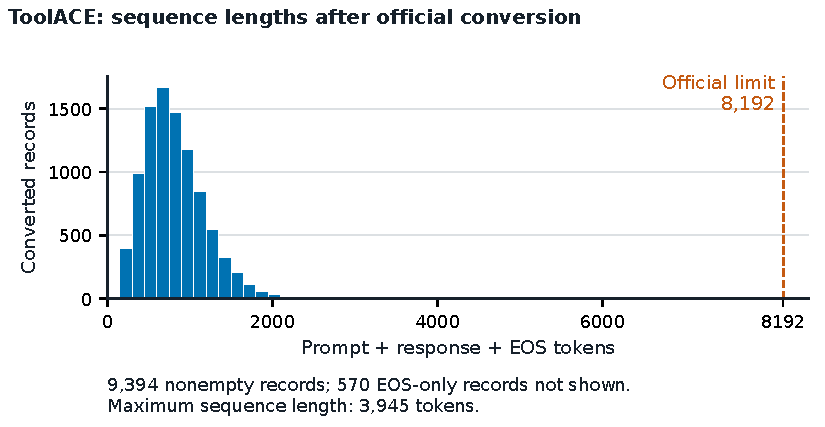
\includegraphics[width=\linewidth]{../figures/toolace_released_lengths.pdf}
\caption{\ToolACELengthCaption}
\label{fig:toolace-lengths}
\end{figure}
\FloatBarrier

\Needspace{4.5in}
\section{Missing-pair analysis}

\begin{figure}[!htbp]
\centering
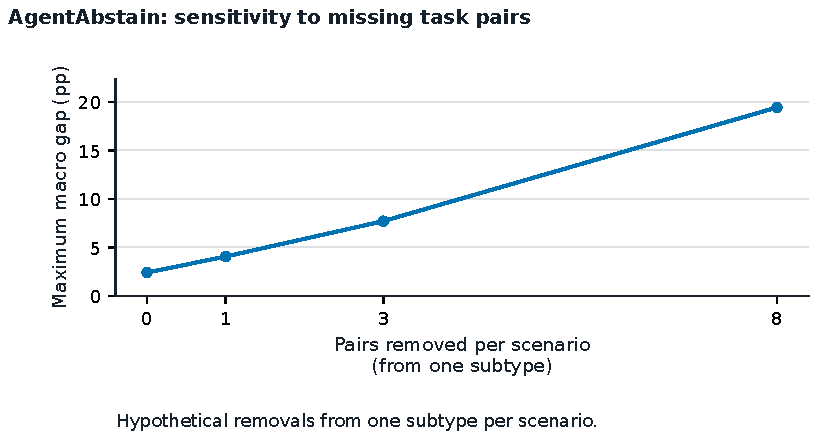
\includegraphics[width=\linewidth]{../figures/agentabstain_missing_pairs.pdf}
\caption{\MissingPairsCaption}
\label{fig:missing-pairs}
\end{figure}
\FloatBarrier

\section{ContractBench comparison}
\begin{table}[!htbp]\centering\small% Requires: booktabs, tabularx, array
\begin{tabularx}{\linewidth}{@{}>{\raggedright\arraybackslash}p{0.20\linewidth}>{\raggedright\arraybackslash}X@{}}
\toprule
Item & Evidence \\
\midrule
Reported result & Qwen3.5-9B, n=99, 56.6\% \\
Released artifact & Qwen3.5-9B, n=99, 0/99 success labels \\
Matches & model name; denominator \\
Not verified & checkpoint; task set; evaluation configuration \\
Trace issue & 3/99 traces report 8,192 output tokens but contain no terminal assistant response \\
Interpretation & 0/99 successes under the repository mapping; correspondence to the reported evaluation remains unresolved \\
\bottomrule
\end{tabularx}

\caption{Reported ContractBench result and released evaluation records for Qwen3.5-9B.}\label{tab:contractbench-comparison}\end{table}\FloatBarrier

\section{Comparison with conventional tests}
Field/type validation accepts AgentPRM's query-history error because observations and actions have the same string type. ContractBench traces can also retain expected field types while omitting a terminal response. ContractBench's existing regression test covers terminal-response logging. The implementation comparison in this paper evaluates the selected AgentPRM, ToolACE, and AgentAbstain behaviors.

\par\noindent\begin{minipage}{\linewidth}
\section{Execution time after contract authoring}
\begin{nonfloatingtable}
\centering
\begin{tabular}{@{}lrr@{}}
\toprule Repository & Median (s) & IQR (s) \\\midrule
AgentPRM & 0.098 & 0.096--0.100 \\
ContractBench & 0.115 & 0.113--0.117 \\
ToolACE & 0.102 & 0.100--0.103 \\
tau-bench & 0.233 & 0.232--0.235 \\
AgentAbstain & 0.393 & 0.385--0.402 \\
\bottomrule\end{tabular}
\caption{Execution time of the original contract invocations, including process startup and reading saved summaries. Median and interquartile range from seven runs per repository on an Apple Silicon CPU. Data acquisition, conversion, and the full ToolACE scan are outside these timings.}
\label{tab:runtime}
\end{nonfloatingtable}

\end{minipage}\par

\section{Repository revisions}
We evaluated AgentPRM at \texttt{e4714717}, ContractBench at \texttt{c50eefee}, ToolACE at \texttt{1156d649}, $\tau$-bench at \texttt{59a200c6}, and AgentAbstain at \texttt{f5812497}. The AgentAbstain dataset revision is \texttt{84222842}. Full commit hashes and the dataset SHA-256 are included in the repository.
\end{document}
